\documentclass{ltjsarticle}
%\usepackage[dvipdfmx]{graphicx}
\usepackage{graphicx}
\usepackage{booktabs}
\usepackage{mathcomp}
\usepackage{array}
\usepackage{mathtools,amssymb}
\usepackage{siunitx}
\usepackage{multirow}
\usepackage{tabularx}
\usepackage{subcaption}
\usepackage{float}
\usepackage{setspace}
\usepackage{abstract}

\title{仮想筋電義手の開発に関する研究}
\author{河合 将暉}
\adviser{戸崎 哲也}

\thispagestyle{empty}
\pagestyle{empty}

\begin{document}
\maketitle

\section{はじめに}
	上肢切断者が筋電義手を装着する際,自在に扱うことができるように
	訓練を行う必要があり,VRシミュレータを用いた訓練効果については
	先行研究\cite{ref:1}で検討されている.本研究では,仮想筋電義手
	3Dモデル(VH:Virtual Hand)のリアリティによる訓練効果に着目し3D
	スキャナで取り込んだVHを用いたVRトレーニングシステムを構成し,
	その見た目によって訓練効果に変化があるかを評価することを目的とする.
	インタフェースを実際の上肢切断者にも使用可能にするため,筋変位
	センサであるFirstVRを用いてVRトレーニングシステムの構成および
	その評価を行った.
\section{解説}
	\subsection{FirstVR}
		FirstVR\cite{ref:2}とは,H2L株式会社が提供する筋変位VRコントローラである.
		コントローラに搭載されているセンサとしては,3軸ジャイロセンサ,
		3軸加速度センサ,3軸磁気センサ,14チャンネルの光学筋変位センサ
		が搭載されている.対応しているOSはiOS/Android OSに対応しており,
		OSとの通信はBLE通信で行われている.

	\subsection{ジェスチャ認識}
		FirstVRではジェスチャを認識することができ,その方式として,
		特定のジェスチャをしている状態の筋変位値を閾値とすることで,
		何もしていない状態とジェスチャを行っている状態を区別して
		認識している.

\section{研究内容}
	\subsection{FirstVRの性能評価手法}
		本研究で構成するシミュレータの入力感度を検証するため,実験協力者として電子工学科5年生の学生31名(男性26名:女性5名)を対象に以下の手順でFirstVRの評価を行う.
		また,ジェスチャ状態は物体保持のアニメーションと同期させるため,じゃんけんのグーのジェスチャを学習させる.
		FirstVRで筋変位を測定した14チャンネル光変位センサの測定値を用いてジェスチャ認識の精度を確認するため,
		各実験協力者・各sample数ごとの評価指標として総変化量$X$を定める.総変化量の算出は測定回数$s = 5$,チャンネル数$r = 14$としてジェスチャ状態で測定した筋変位センサの値を$M_{{s}{r}}$
		とジェスチャしていない状態の筋変位センサの値$N_{r}$とすると式\refeq{eq:originaldata}と示すことができる.
		この評価指標を用いて各sample数ごとに分散を調べ,最適なsample数の検討を行う.
		\begin{equation}
			\label{eq:originaldata}
			X = \frac{1}{5} \sum_{s = 1}^{5} \sum_{r = 0}^{13} |N_{r} - M_{{s}{r}}|
		\end{equation}
		

	\subsection{シミュレータの構成}
		Blenderで処理したVHをUnityにインポートし,入力インターフェースとしてキーボード・マウス
		を用いるPC版と,\,FirstVRを用いるiOS版の2種類を構成した.
		図\refeq{fig:simuraterconst}にシミュレータの構成図を示す.

		\begin{figure}[H]
		\centering
		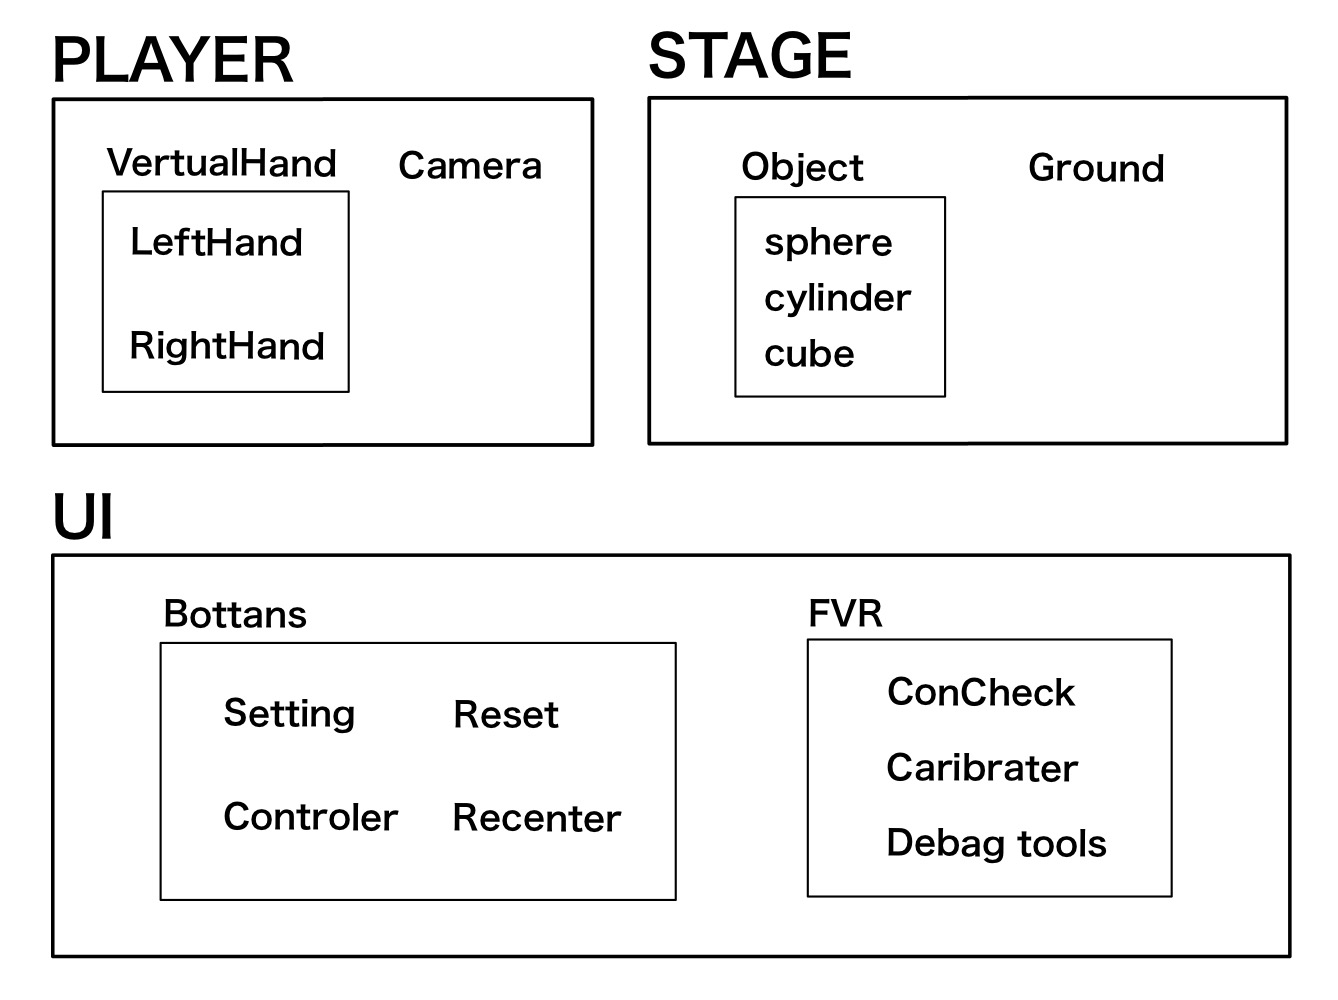
\includegraphics[width = 4cm]{../figs/IMG_0340.jpg}
		\caption{シミュレータ構成図}
		\label{fig:simuraterconst}
		\end{figure}
		\vspace{-30pt}
		
	\subsection{シミュレータの定性評価手法}
		電子工学科5年生の男性11名に協力していただき,\,PC版シミュレータとiOS版シミュレータの2種類の操作説明を説明した後,
		5分程度体験してもらい,各シミュレータにおいての没入感,操作性,応答性の3項目について6段階リッカート尺度を用いた定性評価
		アンケート調査を行う.
		評価点数が高いほどそれぞれの項目において高得点の評価となるように設定し,調査結果に対して分析を行う.

\section{研究結果}
		FirstVRの性能評価用アプリケーションの構成を図\refeq{fig:FirstVRapplication}に示す.
		\begin{figure}[H]
		\centering
		\begin{minipage}{0.45\columnwidth}
		\centering
		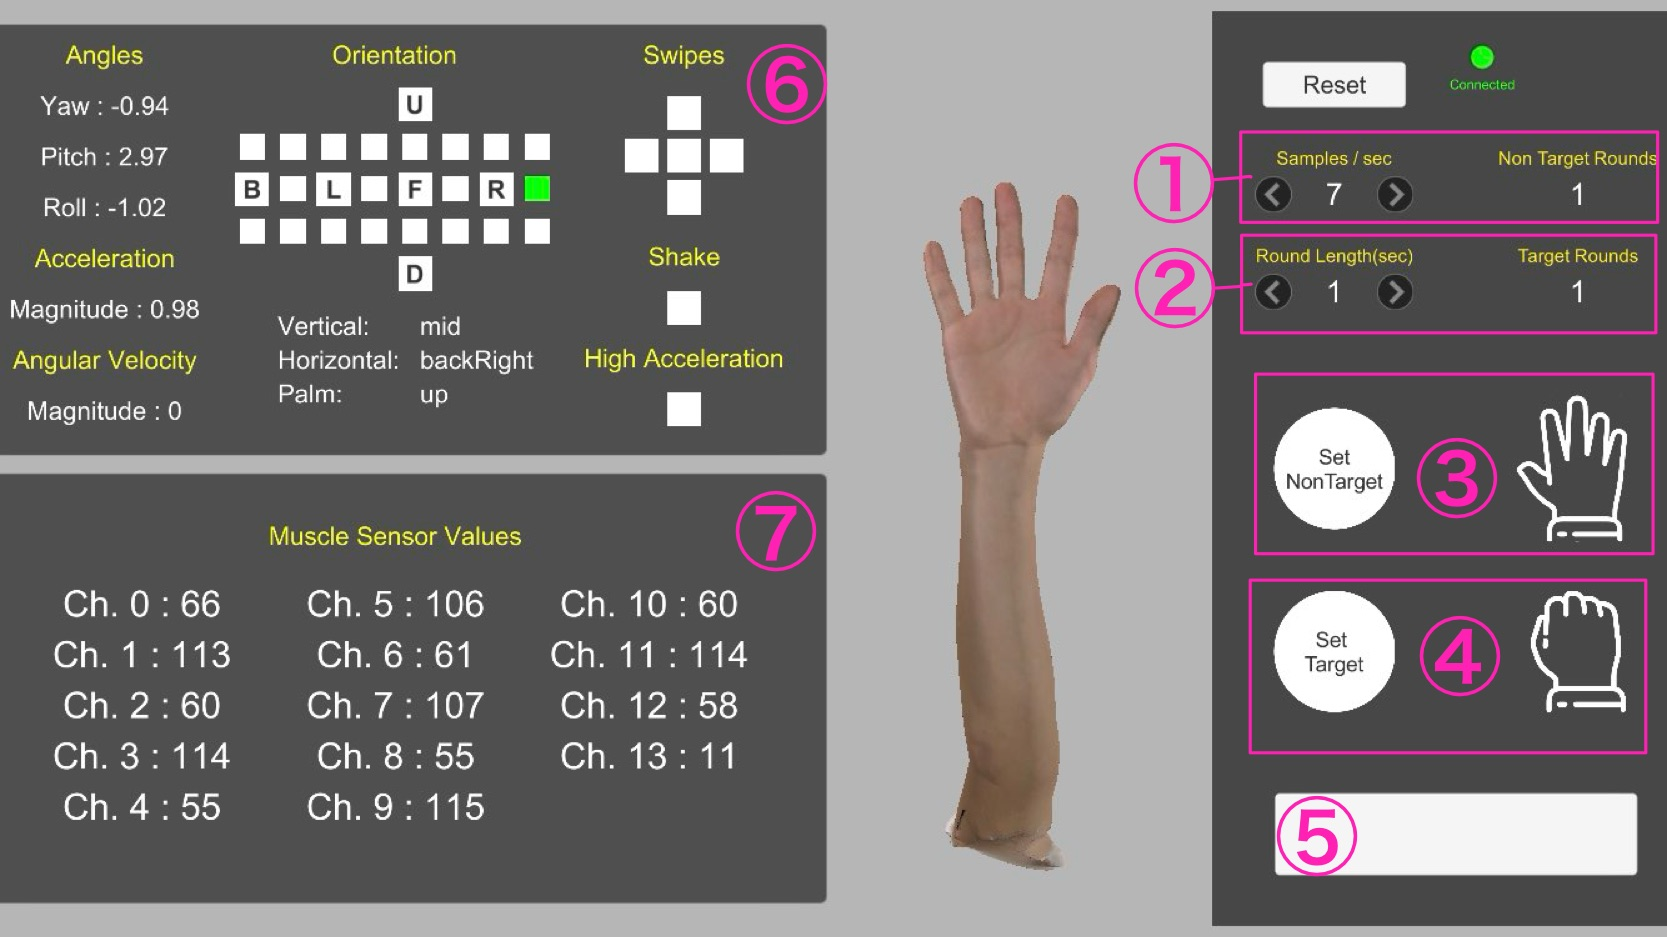
\includegraphics[width = \columnwidth]{../figs/IMG_0345.JPG}
		\subcaption{ジェスチャ未判定時}
		\label{fig:FVRnocalibration}
		\end{minipage}
		\hspace{0.04\columnwidth}
		\begin{minipage}{0.45\columnwidth}
		\centering
		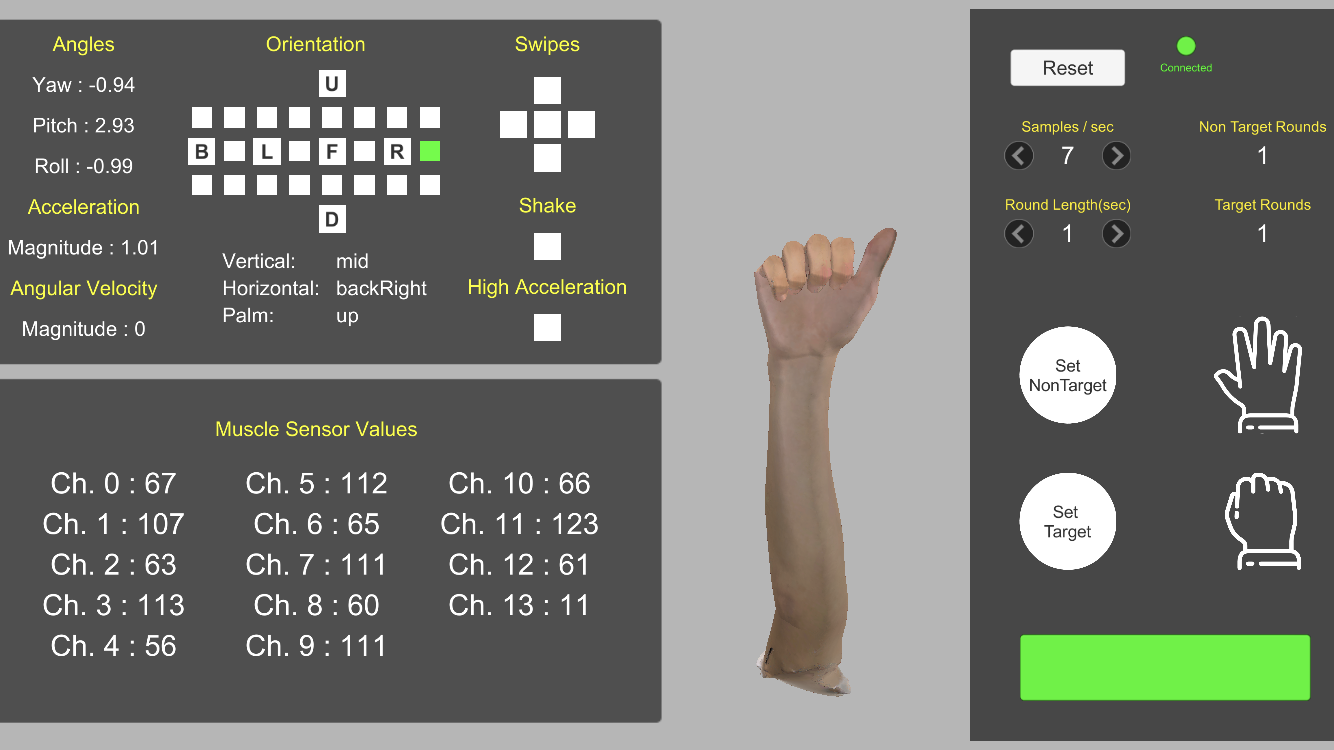
\includegraphics[width = \columnwidth]{../figs/IMG_1867.PNG}
		\subcaption{ジェスチャ判定時}
		\end{minipage}
		\caption{FirstVR性能評価用アプリケーションの構成}
		\label{fig:FirstVRapplication}
		\end{figure}
		\vspace{-15pt}

		10回以上誤検知が起きている実験協力者のデータでは特定のsample数によらずに誤検知が発生しているため,\,sample数によるジェスチャ認識率のデータ
		含めてしまうとノイズによってデータが正しく求められないため除外した.
		各sample数における総変化量の分散を図\refeq{fig:FVRdata}に示す.

		\begin{figure}[H]
		\centering
		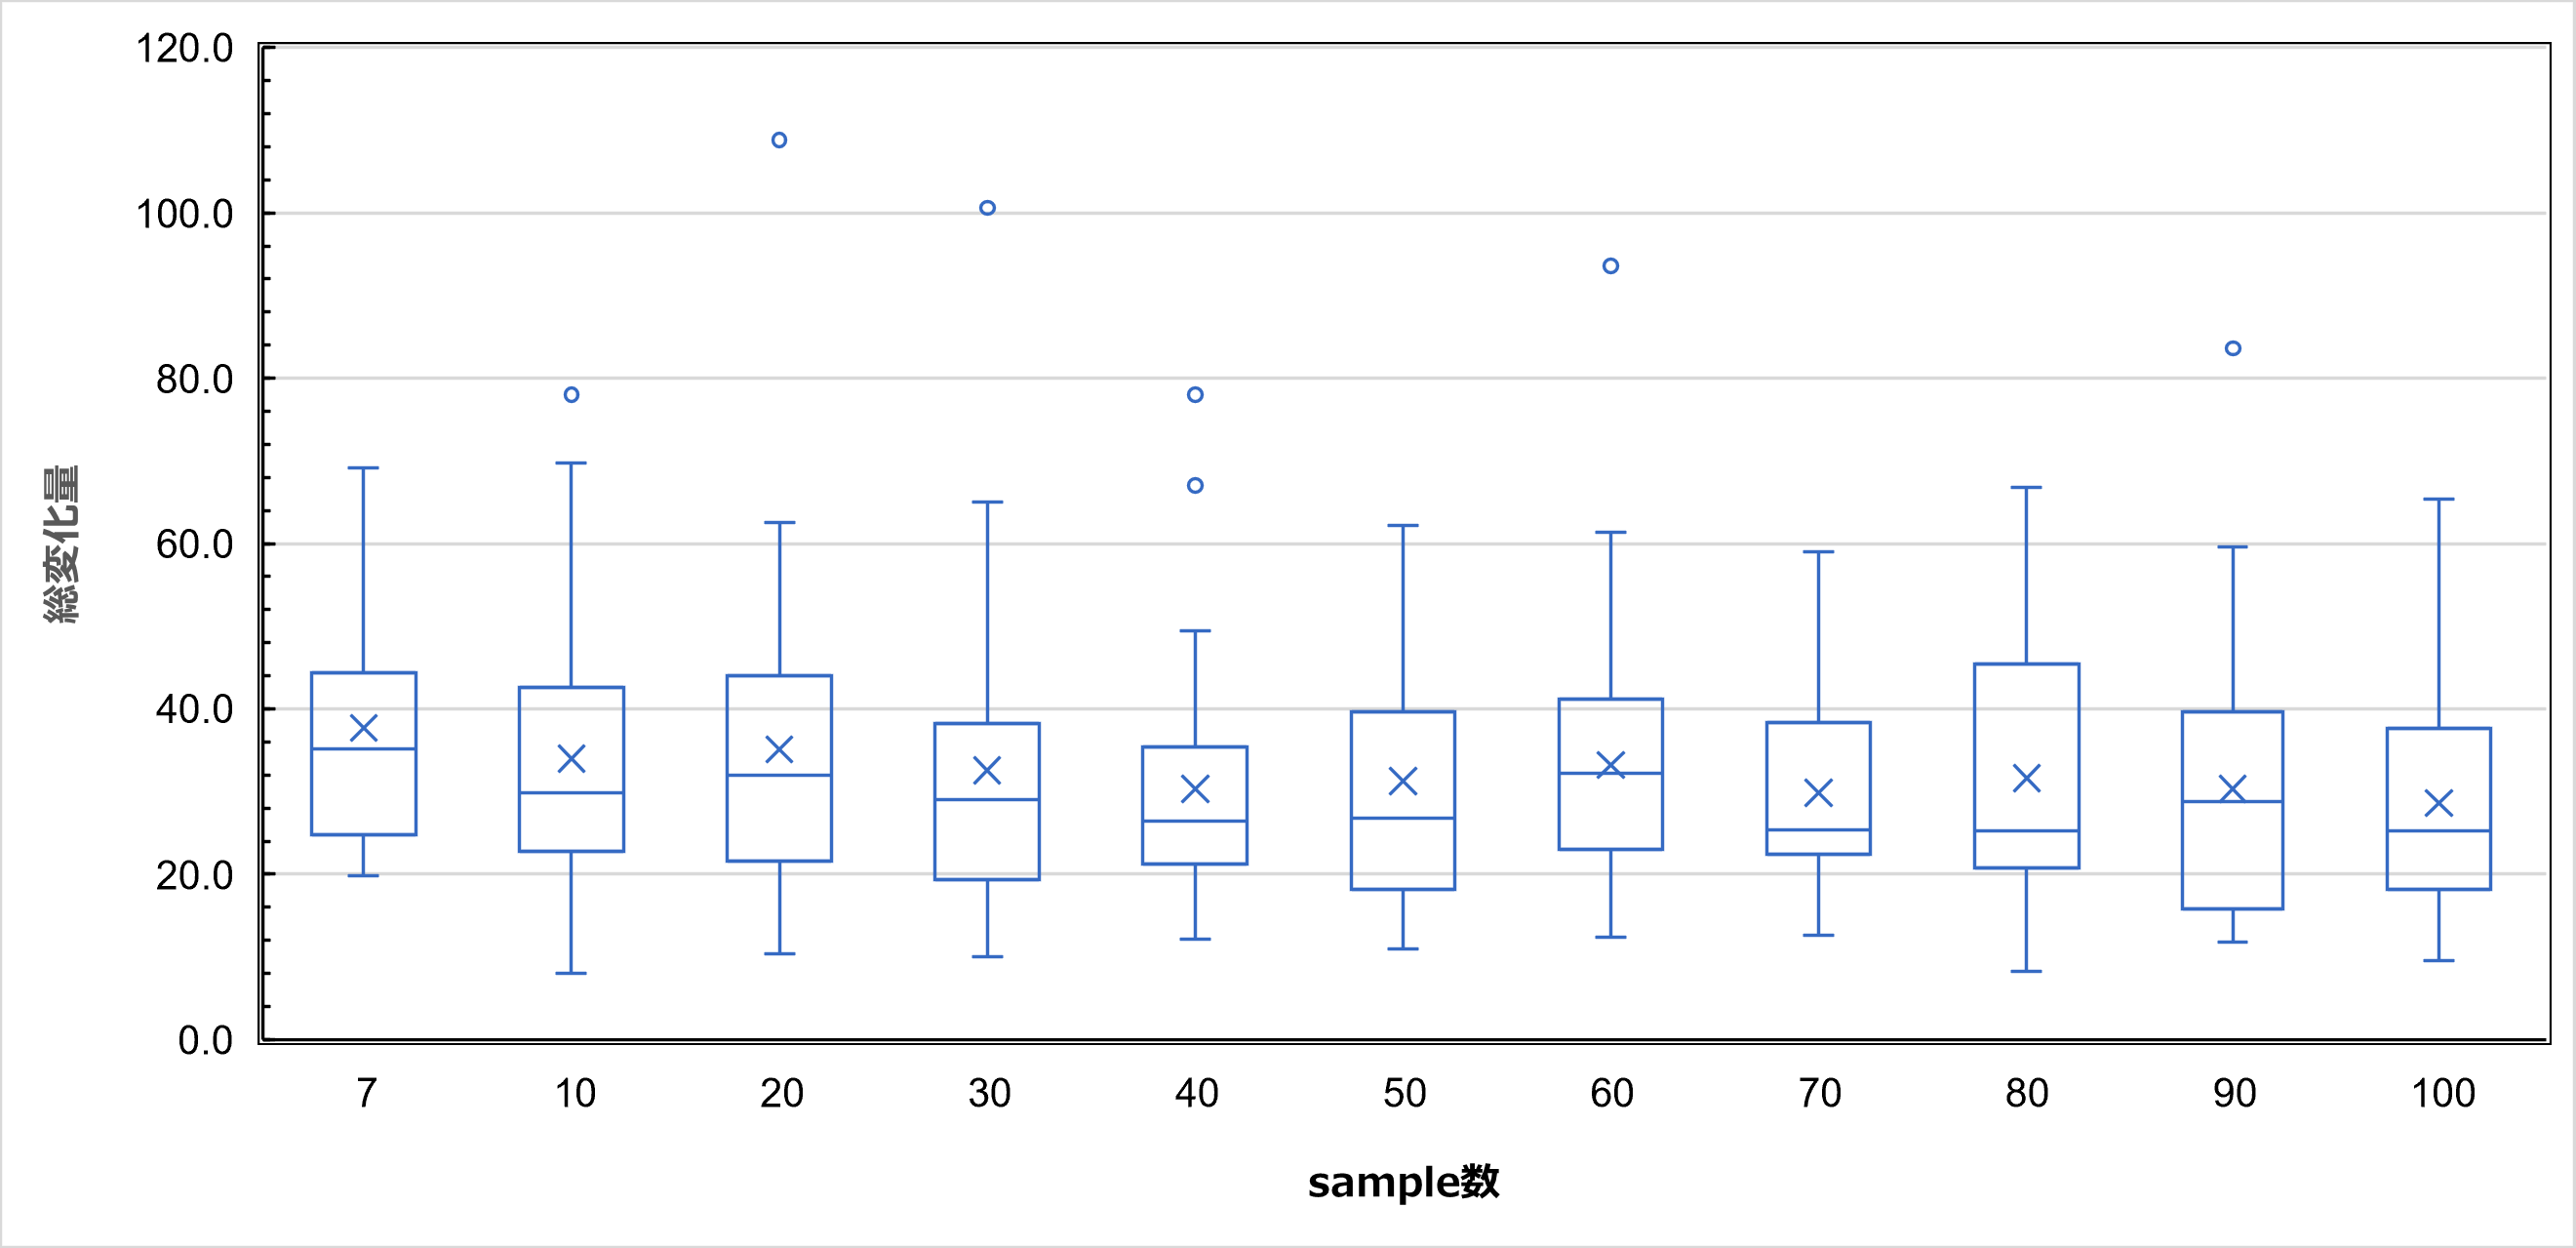
\includegraphics[width = 6cm]{../figs/FVRALL.png}
		\caption{sample数ごとの総変化量分散}
		\label{fig:FVRdata}
		\end{figure}
		\vspace{-15pt}
		図\refeq{fig:FVRdata}より,標本分散はsample70が最も小さく,次いでsample7が分散が少なくなっていることがわかる.
		ここで,\,sample数7,70,100以外のデータは分散がこの3種類よりも比較的大きく,外れ値も含んでいるため,安定して動作していると考えにくい.
		また,この3種類の中で最もシミュレータに対する負荷が小さいデータとしてsample7を選定した.

	\subsection{シミュレータの構成}
		PC版シミュレータの画面構成を図\refeq{fig:PCsimurate}に示す.
		\begin{figure}[H]
		\centering
		\begin{minipage}{0.45\columnwidth}
		\centering
		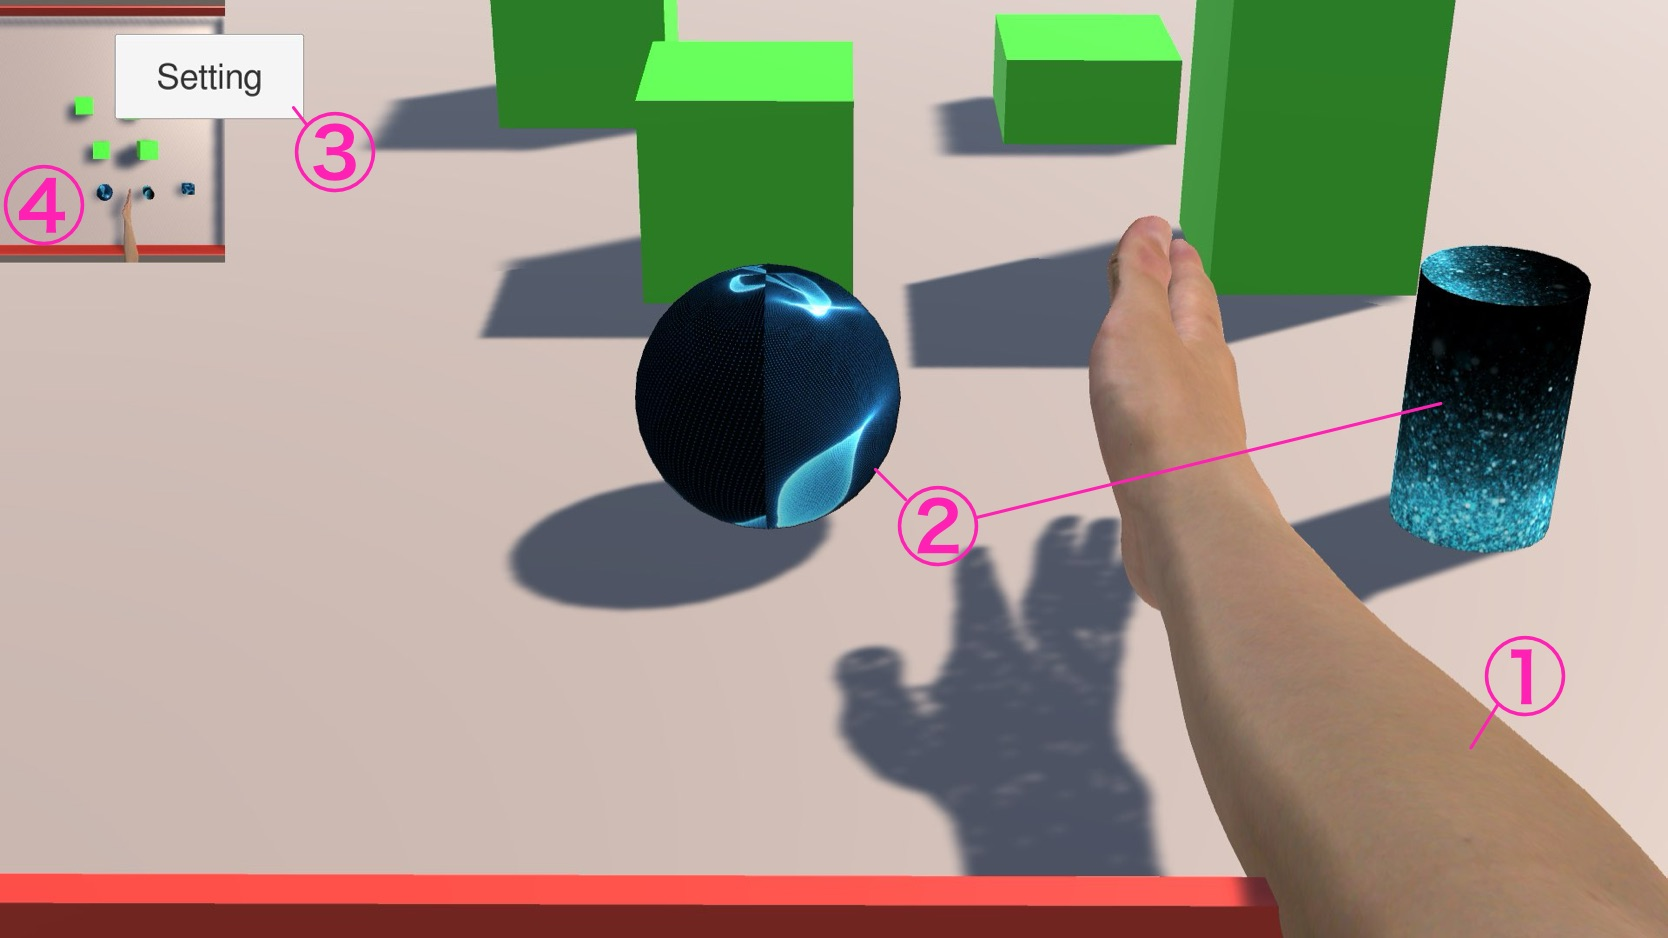
\includegraphics[width = \columnwidth]{../figs/IMG_0341.JPG}
		\subcaption{通常時の構成}
		\end{minipage}
		\hspace{0.04\columnwidth}
		\begin{minipage}{0.45\columnwidth}
		\centering
		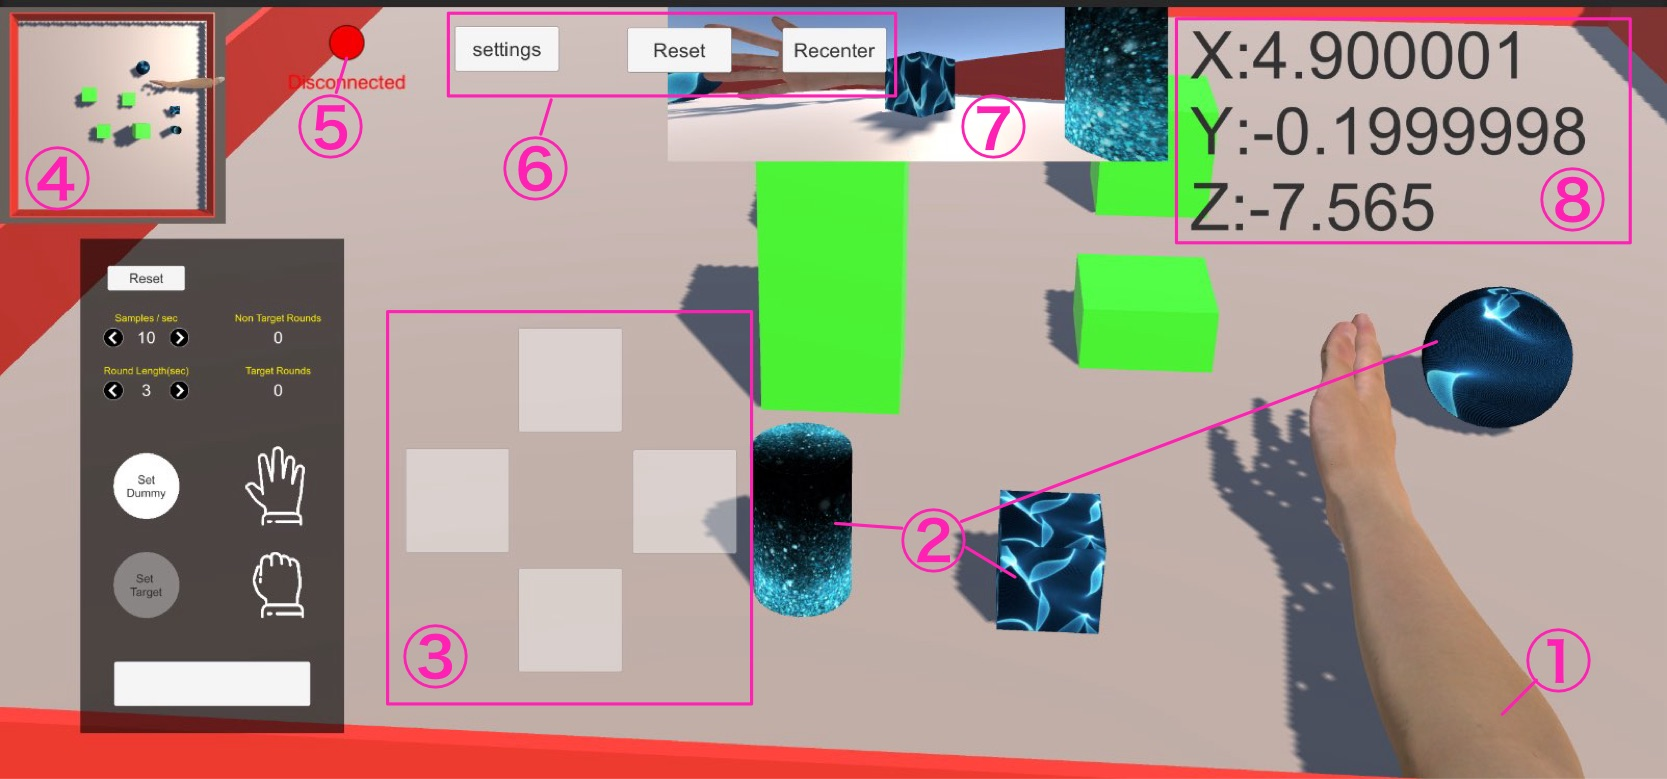
\includegraphics[width = \columnwidth]{../figs/IMG_0344.JPG}
		\subcaption{メニュー起動時の構成}
		\end{minipage}
		\caption{シミュレータの実行画面}
		\label{fig:PCsimurate}
		\end{figure}
		\vspace{-25pt}

	\subsection{シミュレータの定性評価}

		PC版ではキーボード・マウスを入力インターフェースとしているため,
		学習などは必要なく,基本的な操作説明のあとにシミュレータを評価した.
		iOS版ではiPhoneにシミュレータを表示させ,\,FirstVRのジェスチャ認識機能
		によってじゃんけんのグーの状態を学習することでオブジェクト保持ができる.
		この学習が終了してから約5分間シミュレータを評価した.
		次に,アンケート調査の結果を図\refeq{fig:botunyu}~\refeq{fig:tien}に示す.

		\begin{figure}[H]
		\centering
		\begin{minipage}{0.45\columnwidth}
		\centering
		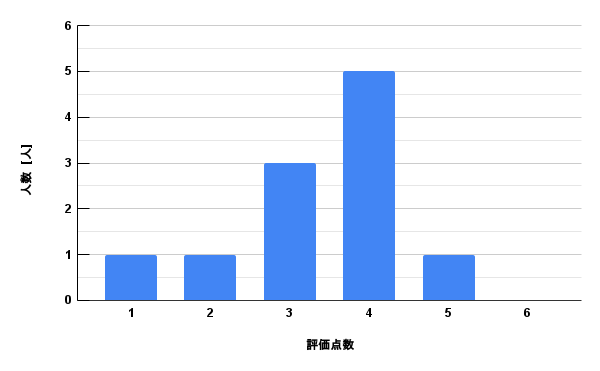
\includegraphics[width = \columnwidth]{../figs/PC-1.png}
		\subcaption{PC版アンケート結果}
		\end{minipage}
		\hspace{0.04\columnwidth}
		\begin{minipage}{0.45\columnwidth}
		\centering
		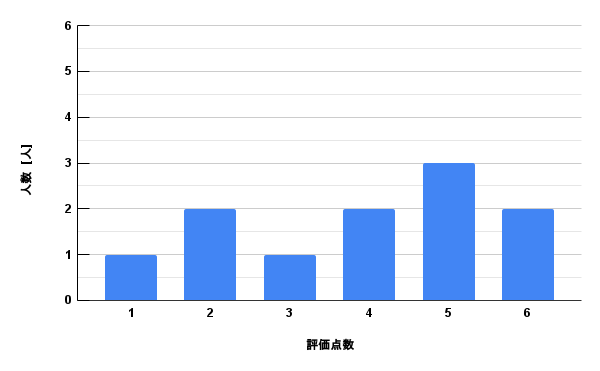
\includegraphics[width = \columnwidth]{../figs/iOS-1.png}
		\subcaption{iOS版アンケート結果}
		\end{minipage}
		\caption{没入感の評価比較}
		\label{fig:botunyu}
		\end{figure}
		\vspace{-15pt}
		
		\begin{figure}[H]
		\centering
		\begin{minipage}{0.45\columnwidth}
		\centering
		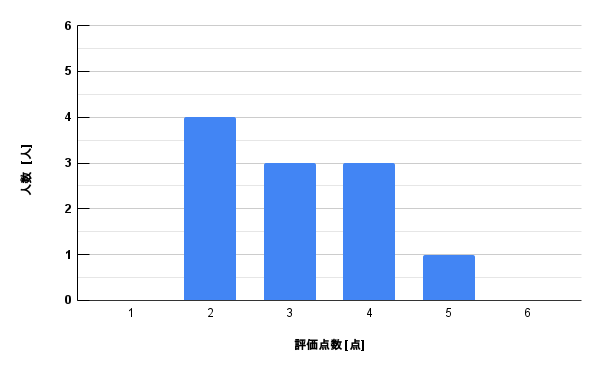
\includegraphics[width = \columnwidth]{../figs/PC-2.png}
		\subcaption{PC版アンケート結果}
		\end{minipage}
		\hspace{0.04\columnwidth}
		\begin{minipage}{0.45\columnwidth}
		\centering
		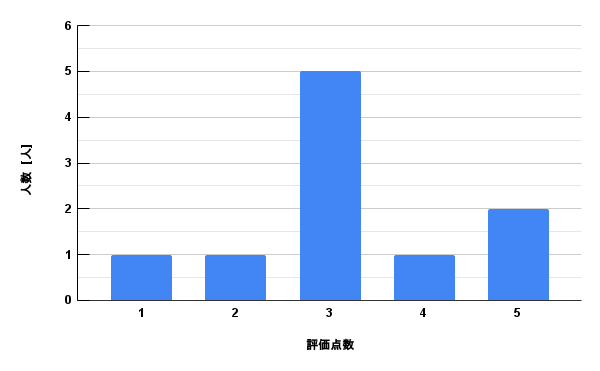
\includegraphics[width = \columnwidth]{../figs/iOS-2.png}
		\subcaption{iOS版アンケート結果}
		\end{minipage}
		\caption{操作性の評価比較}
		\label{fig:sousasei}
		\end{figure}

		\begin{figure}[H]
		\centering
		\begin{minipage}{0.45\columnwidth}
		\centering
		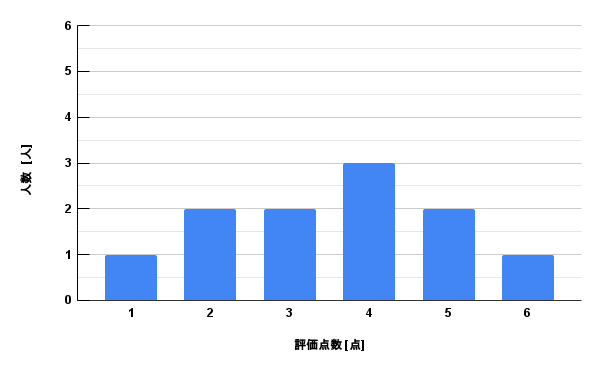
\includegraphics[width = \columnwidth]{../figs/PC-3.png}
		\subcaption{PC版アンケート結果}
		\end{minipage}
		\hspace{0.04\columnwidth}
		\begin{minipage}{0.45\columnwidth}
		\centering
		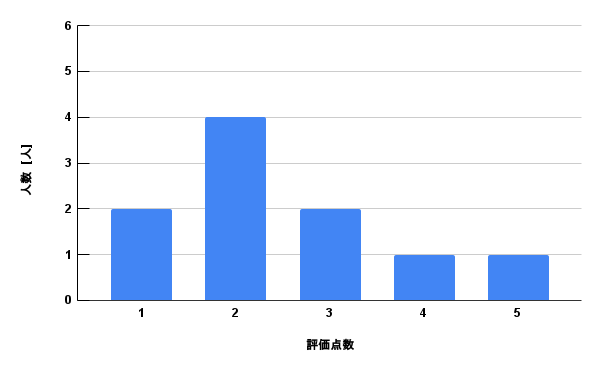
\includegraphics[width = \columnwidth]{../figs/iOS-3.png}
		\subcaption{iOS版アンケート結果}
		\end{minipage}
		\caption{操作遅延の評価比較}
		\label{fig:tien}
		\end{figure}
		\vspace{-15pt}

		

\section{おわりに}
	本研究ではPC版のシミュレータとiOS版のシミュレータの2種類を作製し,健常者に
	体験してもらい,その定性評価を行うことでFirstVRを用いたシミュレータの方が没入感
	が高い傾向があることを示した.しかし,操作性の点では多少の優位性を得ることができたが,
	装着者各個人による評価点の分散が大きいことが課題となった.また,遅延に関してもPC版の方が遅延が少ないという課題点も見つかった.
	そのうえ,表示するモニターの違いで没入感が違ったという意見も挙げられており,
	実験方法を再検討する必要がある.

\begin{thebibliography}{99}%参考文献
	\begin{spacing}{0.8}

		\bibitem{ref:1}
			H2L.Inc.,Tokyo106-0032,Japan;satoshi.hosono@h2l.jp
		\bibitem{ref:2}
			Tamon Miyake, etal``Gait Phase Detection Based on Muscle Deformation
			with Static Standing-Based Calibration''.
			MDPI. 2021 Feb

	\end{spacing}
\end{thebibliography}
\end{document}